\documentclass[english]{beamer}
\usepackage[english]{babel}
\usepackage{bookmark}
\usepackage[utf8]{inputenx}
\usepackage[T1]{fontenc}      % Font encoding
\usepackage{lmodern}          % lmodern font, correctly copyable characters in pdf
\usepackage{microtype}
\usepackage{graphicx}
\usepackage{subcaption}

\usetheme[
  bullet=circle,                  % Use circles instead of squares for bullets
  titleline=false,                % Show a line below the frame
  alternativetitlepage=true,      % Use the fancy title
  titlepagelogo=logo-sapienza,    % Logo for the first slide
  watermark=watermark-diag,   % Watermark used in every slide
  watermarkheight=20px,           % Desired height of the watermark
  watermarkheightmult=6,          % Watermark image is actually x times bigger
  displayauthoronfooter=true,     % Display author name in the footer
]{Roma}
\watermarkoff
\author{Giuseppina Iannotti, 1938436\\Davide Marincione, 1927757}
\title{A multimodal interface for chess}
\subtitle{How we made people gesticulate and scream at their computers}
\institute{Sapienza, University of Rome}
\date{A. Y. 2023 - 2024}

\begin{document}

\begin{frame}[t, plain]
\titlepage
\end{frame}

\section{Introduction}
\begin{frame}[c]{The Idea}
    Remember this?
    \begin{figure}
        \centering
        \includegraphics[width=.85\textwidth]{images/wizard_chess.png}
        \caption{Wizard's Chess, Harry Potter and the Philosopher's Stone}
    \end{figure}
\end{frame}

\begin{frame}[c]{The Idea 2}
    Know this feeling?
    \begin{figure}
        \centering
        \includegraphics[width=.7\textwidth]{images/stock_hand.jpeg}
        \caption{Some stock image of an hand holding a chess piece.}
    \end{figure}
\end{frame}

\section{Code, Graphx, \& Sound}
\begin{frame}{Before that}
    \begin{columns}[T]
        \begin{column}{.5\textwidth}
            We have to get from here\dots
            \begin{figure}
                \centering
                \includegraphics[width=.65\textwidth]{images/empty_set.png}
                \caption{What we have.}
            \end{figure}
        \end{column}
        \begin{column}{.5\textwidth}
            To here!
            \begin{figure}
                \centering
                \includegraphics[width=.9\textwidth]{images/gui_example.png}
                \caption{What we want.}
            \end{figure}
        \end{column}
    \end{columns}
\end{frame}

\begin{frame}{We need some OOP}
    \begin{figure}
        \centering
        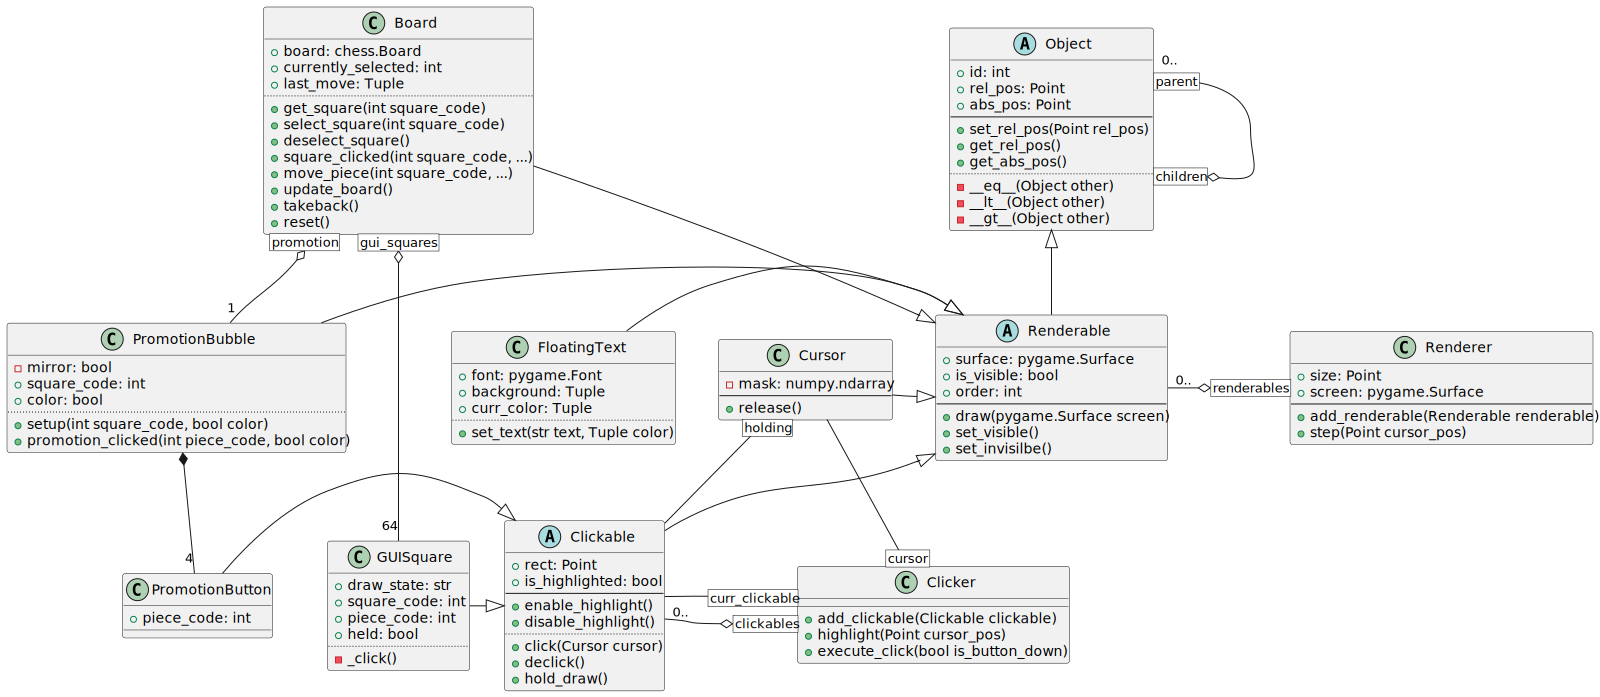
\includegraphics[width=.98\textwidth]{images/uml.pdf}
        \caption{Class diagram of the game's elements}
    \end{figure}
\end{frame}

\begin{frame}{A bit in detail 1}
    \begin{columns}[T]
        \begin{column}{.5\textwidth}
            The \texttt{Renderer}\dots draws \texttt{Renderables}!
            \begin{enumerate}
                \item Keeps track of them.
                \item Draws them based on each object's \texttt{order} attribute.
                \item Draws them only if they are set to visible.
            \end{enumerate}
        \end{column}
        \begin{column}{.5\textwidth}
            The \texttt{Clicker}:
            \begin{enumerate}
                \item Keeps track of the \texttt{Clickable}s.
                \item Highlights the current \texttt{Clickable}, calls its click/declick method.
                \item Drives hold/release with \texttt{Cursor}.
            \end{enumerate}
        \end{column}
    \end{columns}
\end{frame}

\begin{frame}{A bit in detail 2}
    \begin{columns}[T]
        \begin{column}{.5\textwidth}
            Our \texttt{Cursor} is this neat thing:
            \begin{figure}
                \centering
                \includegraphics[width=.98\textwidth]{images/cursor_comparison.png}
                \caption{Our \texttt{Cursor}.}
            \end{figure}
        \end{column}
        \begin{column}{.5\textwidth}
            It is simple, but we are pretty happy about it:
            \begin{enumerate}
                \item It is extremely visible, because of the dynamic color
                \begin{equation*}
                    c^* = (c + 128)\ \mathrm{mod}\ 256.
                \end{equation*}
                \item It can hold pieces.
                \item Being stylistically different might have helped!
            \end{enumerate}
        \end{column}
    \end{columns}
\end{frame}

\begin{frame}{A bit in detail 3}
    \begin{columns}
        \begin{column}{.5\textwidth}
            The \texttt{Board}:
            \begin{enumerate}
                \item Wraps a \texttt{chess.Board} object (and all its complicated chess logic).
                \item Handles the state of all the \texttt{GUISquare} and that of the \texttt{PromotionBubble}.
                \item Plays audio when moves are done!
            \end{enumerate}
        \end{column}
        \begin{column}{.5\textwidth}
            \begin{figure}
                \centering
                \includegraphics[width=.4\textwidth]{images/check_coloring.png}
                \includegraphics[width=.4\textwidth]{images/moves_coloring.png}
                \caption{Examples of \texttt{GUISquare} states}
                \includegraphics[width=.65\textwidth]{images/promotion_ex.png}
                \caption{What \texttt{PromotionBubble} looks like}
            \end{figure}
        \end{column}
    \end{columns}
\end{frame}

\begin{frame}{The main loop}
    All of this runs on the main thread, within the loop:

    \begin{enumerate}
        \item Update cursor with latest mouse or hand position.
        \item \texttt{clicker.highlight(cursor\_pos)}.
        \item Resolve events, such as mouse clicks, key presses (quit game, takebacks), and moves done (for the AI).
        \item Resolve voice commands.
        \item \texttt{renderer.step()}.
        \item Run metrics recorder.
    \end{enumerate}
\end{frame}

\section{Voice commands}
\begin{frame}{Dragonfly? What's that?}
\end{frame}

\begin{frame}{Rules 1}
\end{frame}

\begin{frame}{Rules 2}
\end{frame}

\begin{frame}{Validating commands}
\end{frame}


\section{Hand tracking \& gestures}
\begin{frame}{Good ol' mediapipe}
\end{frame}

\begin{frame}{'Hand'made normalization}
\end{frame}

\begin{frame}{Gesture recognition}
\end{frame}

\begin{frame}{Hand2Cursor mapping}
\end{frame}

\section{Experiments}
\begin{frame}{Recording users}
\end{frame}

\begin{frame}{Some metrics}
\end{frame}

\begin{frame}{Results 1}
\end{frame}

\begin{frame}{Results 2}
\end{frame}


\begin{frame}{Conclusions}
\end{frame}

\end{document}